\documentclass[tikz,convert={outext=.svg,command=\unexpanded{pdf2svg \infile\space\outfile}},multi=false]{standalone}
%\usepackage{tikz}

% tikz setup
\usetikzlibrary{automata, positioning, arrows}

\tikzset{%
    ->,
    >=stealth',
    node distance=2cm,
    .every state/.style={thick, fill=gray!10},
    initial text=$ $,
}

\begin{document}
    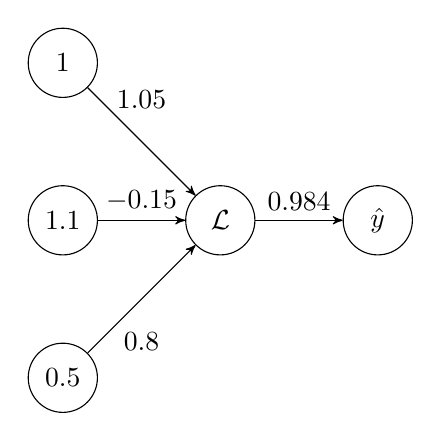
\begin{tikzpicture}
        \node[state] (b) {$1$};
        \node[state, below of=b] (x1) {$1.1$};
        \node[state, below of=x1] (x2) {$0.5$};
        \node[state, right of=x1] (L) {$\mathcal{L}$};
        \node[state, right of=L] (y) {$\hat{y}$};

        \draw (b) edge[above] node[yshift=3mm] {$1.05$} (L)
        (x1) edge[above] node[] {$-0.15$} (L)
        (x2) edge[below] node[yshift=-3mm] {$0.8$} (L)
        (L) edge[above] node[] {$0.984$} (y)
        ;
    \end{tikzpicture}
\end{document}